\documentclass[10pt,letterpaper]{article}
\usepackage[T1]{fontenc}
\usepackage[utf8]{inputenc}
\usepackage{textcomp}
\usepackage{amsmath,amssymb}
\usepackage[margin=0.7in]{geometry}
\usepackage{graphicx,longtable,booktabs,array,calc}
\usepackage{fvextra}
\usepackage[hidelinks]{hyperref}
\usepackage[expansion=false]{microtype}
\usepackage{etoolbox}
\usepackage{caption}
\usepackage{float}
\floatplacement{figure}{H}
\captionsetup{justification=centering,singlelinecheck=false,labelformat=empty,font=it}
\setlength{\LTpre}{4pt}
\setlength{\LTpost}{6pt}
\setcounter{tocdepth}{2}
\setcounter{secnumdepth}{0}
\renewcommand{\contentsname}{Table of contents}
\hypersetup{pdftitle={Project 2: Cache \& Memory Performance Profiling},pdfauthor={Rashid Shabab}}
\widowpenalty=10000
\clubpenalty=10000
\setlength{\parindent}{0pt}
\setlength{\parskip}{6pt}
\setlength{\tabcolsep}{4pt}
\renewcommand{\arraystretch}{1.18}
\emergencystretch=3em
\AtBeginEnvironment{longtable}{\footnotesize}
\AtBeginEnvironment{Highlighting}{\footnotesize}
\providecommand{\tightlist}{\setlength{\itemsep}{0pt}\setlength{\parskip}{0pt}}
\providecommand{\pandocbounded}[1]{#1}
\usepackage{fancyvrb}
\DefineVerbatimEnvironment{verbatim}{Verbatim}{fontsize=\footnotesize,breaklines}
\begin{document}
\begin{titlepage}
\thispagestyle{empty}
\centering
\vspace*{1.2in}
{\Large\bfseries ECSE 6320\par}
\vspace{0.3in}
{\Large Advanced Computer Systems\par}
\vspace{0.9in}
{\LARGE\bfseries Project 2: Cache \& Memory Performance Profiling\par}
\vspace{0.9in}
{\large Submitted by Rashid Shabab\par}
\vfill
\end{titlepage}
\setcounter{page}{2}
\tableofcontents
\clearpage
\hypertarget{introduction}{%
\subsection{1. Introduction}\label{introduction}}

In this project, I measured the cache and memory hierarchy
of an AMD Ryzen 9 9950X (Zen 5) running CachyOS Linux. Intel
MLC only partly works on AMD and several of its modes need
root, which I did not have, so I used three small C
benchmarks written for this project instead: a pointer-chase
latency benchmark (\texttt{pchase}), a streaming bandwidth
benchmark (\texttt{bwbench}) and a SAXPY kernel
(\texttt{saxpy}). All three pin themselves to a core,
control the page size, read hardware counters around the
timed loop only, and check their own correctness before
timing.

\begin{longtable}[]{@{}
  >{\raggedright\arraybackslash}p{(\columnwidth - 4\tabcolsep) * \real{0.3333}}
  >{\raggedright\arraybackslash}p{(\columnwidth - 4\tabcolsep) * \real{0.3333}}
  >{\raggedright\arraybackslash}p{(\columnwidth - 4\tabcolsep) * \real{0.3333}}@{}}
\toprule\noalign{}
\begin{minipage}[b]{\linewidth}\raggedright
Metric
\end{minipage} & \begin{minipage}[b]{\linewidth}\raggedright
Result
\end{minipage} & \begin{minipage}[b]{\linewidth}\raggedright
Setting
\end{minipage} \\
\midrule\noalign{}
\endhead
\bottomrule\noalign{}
\endlastfoot
L1 / L2 / L3 load-to-use latency & 4.0 / 14.0 / 47.3 cycles
& Random pointer chase, 32 KiB / 512 KiB / 16 MiB \\
DRAM latency & 97.9 ns (559 cycles at 5.71 GHz) & Random
pointer chase, 1 GiB \\
Effective L3 capacity for one core & 32 MiB (not the chip's
64 MiB) & Working-set sweep \\
Single-core DRAM bandwidth & 54.1 GB/s sequential read; 4.3
GB/s random & 1 GiB, 1 thread \\
Single-core knee & $\sim$48 misses in flight,
$\sim$26 GB/s random; latency 99 $\rightarrow$ 159 ns at 64 &
1--64 independent chains \\
Loaded latency & 101 ns idle $\rightarrow$ 423 ns with one streaming
core (55 GB/s) & Probe on CPU 15 \\
TLB miss cost (4 KiB pages) & 42--64 cycles per miss,
growing with region size & One access per page, 64 MiB--1
GiB \\
\end{longtable}

These were the main findings:

\begin{itemize}
\tightlist
\item
  The latency staircase steps exactly at the documented
  capacities: 48 KiB (L1), 1 MiB (L2) and 32 MiB (one CCD's
  L3). In cycles, cache latency is unaffected by the clock;
  in nanoseconds it is not, because the core ran at either
  4.37 GHz or 5.71 GHz depending on the run.
\item
  One core can keep about 48 independent misses in flight
  before latency rises faster than throughput. Little's Law
  ties the benchmarks together: random SAXPY implies
  $\sim$34 misses in flight, matching the 32-chain
  point of the chain sweep.
\item
  Near memory saturation, a 15\% rise in background
  bandwidth (48 $\rightarrow$ 55 GB/s) nearly tripled the latency of an
  unrelated load (148 $\rightarrow$ 423 ns).
\item
  Writes cost about twice their bytes in DRAM traffic
  (read-for-ownership plus write-back). Counting that, total
  traffic stayed at 43--54 GB/s for every read/write mix.
\item
  With 4 KiB pages, the TLB covers roughly 14 MiB; past
  that, every access needs a page walk that costs about one
  L3 hit.
\item
  Miss counters can mislead: sequential SAXPY slowed down
  12$\times$ from L1 to DRAM with almost no L2 demand misses,
  because the prefetchers turned the misses into hits.
\end{itemize}

\hypertarget{grading-rubric-coverage}{%
\subsection{2. Grading rubric
coverage}\label{grading-rubric-coverage}}

\begin{longtable}[]{@{}
  >{\raggedright\arraybackslash}p{(\columnwidth - 2\tabcolsep) * \real{0.5000}}
  >{\raggedright\arraybackslash}p{(\columnwidth - 2\tabcolsep) * \real{0.5000}}@{}}
\toprule\noalign{}
\begin{minipage}[b]{\linewidth}\raggedright
Rubric category (points)
\end{minipage} & \begin{minipage}[b]{\linewidth}\raggedright
Where it is covered
\end{minipage} \\
\midrule\noalign{}
\endhead
\bottomrule\noalign{}
\endlastfoot
Zero-queue baselines (25) & §4: per-level table in ns and
cycles with the measured clock, min--max over 10 runs,
caveats \\
Pattern / granularity / RW sweeps (35) & §6 (seq vs random $\times$
64/256/1024 B, latency and bandwidth), §7 (four mixes, 1 and
16 threads) \\
Throughput--latency knee (35) & §8: chain sweep (1--64),
knee, diminishing returns, Little's Law, loaded latency \\
Working-set / cache / TLB analysis (35) & §5 (staircase,
AMAT), §9 (SAXPY counters vs runtime, correlations), §10
(dTLB counters, 4 KiB vs 2 MiB) \\
Experimental rigor (25) & §3: pinning, warm-up, repetitions,
in-process counters, self-validation, recorded environment,
\texttt{membench.py} \\
AI-use transparency and pitfall (15) & §11 (six pitfalls,
each demonstrated with data), §16 (AI-use note) \\
Report quality (15) & Figures with units and min--max bars,
§12 anomalies, §13 limitations \\
\end{longtable}

\hypertarget{methodology}{%
\subsection{3. Methodology}\label{methodology}}

\hypertarget{environment}{%
\subsubsection{3.1 Environment}\label{environment}}

\begin{longtable}[]{@{}
  >{\raggedright\arraybackslash}p{(\columnwidth - 2\tabcolsep) * \real{0.5000}}
  >{\raggedright\arraybackslash}p{(\columnwidth - 2\tabcolsep) * \real{0.5000}}@{}}
\toprule\noalign{}
\begin{minipage}[b]{\linewidth}\raggedright
Item
\end{minipage} & \begin{minipage}[b]{\linewidth}\raggedright
Value
\end{minipage} \\
\midrule\noalign{}
\endhead
\bottomrule\noalign{}
\endlastfoot
CPU & AMD Ryzen 9 9950X (Zen 5, family 26 model 68), 16
cores / 32 threads, 1 socket \\
Caches & L1d 48 KiB/core (12-way, 64 sets), L2 1 MiB/core
(16-way), L3 32 MiB per CCD $\times$ 2 (16-way), 64 B lines \\
Topology & CCD 0 = CPUs 0--7, CCD 1 = CPUs 8--15; SMT
siblings 16--31; 1 NUMA node \\
Memory & 60 GiB DRAM; speed grade and channel count not
readable without root (unknown) \\
OS / kernel & CachyOS, Linux 7.3.0-2-cachyos \\
Frequency & \texttt{amd-pstate-epp} driver,
\texttt{powersave} governor, EPP
\texttt{balance\_performance}, boost on; not changeable (no
root). Observed 4.37 or 5.71 GHz during runs \\
SMT & On; the sibling of the measuring core (CPU 18 for CPU
2) was left idle \\
Pages & Transparent huge pages \texttt{always}; each
benchmark sets 4 KiB or 2 MiB pages explicitly with
\texttt{madvise} \\
Compiler & GCC 16.2.1; \texttt{pchase}
\texttt{-O2\ -march=native}, \texttt{bwbench} and
\texttt{saxpy} \texttt{-O3\ -march=native} \\
Counters & \texttt{perf\_event\_open} inside the benchmarks
(user space only, \texttt{perf\_event\_paranoid} = 2); perf
7.2.11 for spot checks \\
Access & Shared lab workstation over SSH, standard user, no
root; load average 0.06--0.72 at session starts \\
\end{longtable}

Every result session also stores a full environment snapshot
(\texttt{env.txt}) and a \texttt{manifest.json} with the
exact commands, compiler and perf versions, timestamps and
the hypothesis.

\hypertarget{benchmarks-and-validation}{%
\subsubsection{3.2 Benchmarks and
validation}\label{benchmarks-and-validation}}

\textbf{\texttt{pchase} (latency).} Builds a chain of
pointers through a buffer in shuffled order, so each load's
address comes from the previous load and the prefetchers
cannot predict it. With \emph{k} independent chains walked
in turn, up to \emph{k} misses are in flight. Before timing,
the program walks every chain once and checks that it is a
single cycle that visits each node exactly once. The chase
loops are generated with one register variable per chain;
\texttt{make\ check-asm} confirms that the one-chain loop is
a bare \texttt{mov\ (\%rax),\%rax}. It reports ns, cycles,
the actual clock, and L1D and dTLB misses per load.

\textbf{\texttt{bwbench} (bandwidth).} Streams over 64 B
chunks with independent accesses, so many misses overlap. It
sets the stride, the order (sequential or shuffled), the
read share (reads sum a line, writes store a line) and the
number of pinned threads, each with its own region. All
threads start at a barrier.

\textbf{\texttt{saxpy} (cache-miss impact).}
\texttt{y\ =\ a$\cdot$x\ +\ y} in float, either in order
(vectorized: GCC emits 256-bit \texttt{vfmadd213ps}) or
through a shuffled index. One pass is checked against a
double-precision scalar reference before timing. It reports
time, cycles, IPC and L1D, L2 and dTLB misses per element.

\textbf{Sanity checks against known values.} L1 measured
exactly 4.0 cycles and L2 exactly 14.0 cycles, matching
commonly reported Zen 5 latencies. The L1D-miss counter in
sequential SAXPY reads exactly 0.125 per element, which is
the expected 2 lines / 16 floats. The \texttt{perf} L2
counters in §10 counted exactly 3 $\times$ 20.97 M accesses for 3 $\times$
20.97 M loads.

\hypertarget{procedure-and-statistics}{%
\subsubsection{3.3 Procedure and
statistics}\label{procedure-and-statistics}}

All runs went through \texttt{scripts/membench.py}, which
saves each experiment to
\texttt{results/raw/\textless{}experiment\textgreater{}/\textless{}session\textgreater{}/}.
Single-thread runs were pinned to CPU 2. Each point ran a
200 ms busy warm-up and one untimed pass over the working
set, then 5 timed repetitions (10 for the baselines). Plots
show the \textbf{median} with bars spanning
\textbf{min--max} across repetitions. I used the median
because the first repetition of a point was sometimes slower
while the clock ramped up. Pattern, read/write, TLB and two
of the three working-set sessions ran in shuffled point
order.

\hypertarget{pre-experiment-hypotheses}{%
\subsubsection{3.4 Pre-experiment
hypotheses}\label{pre-experiment-hypotheses}}

The hypotheses below were written into \texttt{membench.py}
before running; each session's \texttt{manifest.json} stores
the one in effect. The outcome is summarized here and
discussed in each section.

\begin{longtable}[]{@{}
  >{\raggedright\arraybackslash}p{(\columnwidth - 4\tabcolsep) * \real{0.3333}}
  >{\raggedright\arraybackslash}p{(\columnwidth - 4\tabcolsep) * \real{0.3333}}
  >{\raggedright\arraybackslash}p{(\columnwidth - 4\tabcolsep) * \real{0.3333}}@{}}
\toprule\noalign{}
\begin{minipage}[b]{\linewidth}\raggedright
Experiment
\end{minipage} & \begin{minipage}[b]{\linewidth}\raggedright
Hypothesis
\end{minipage} & \begin{minipage}[b]{\linewidth}\raggedright
Outcome
\end{minipage} \\
\midrule\noalign{}
\endhead
\bottomrule\noalign{}
\endlastfoot
Baselines & L1 $\sim$4, L2 $\sim$14, L3
$\sim$50 cycles, DRAM 80--100 ns & Supported: 4.0,
14.0, 47.3 cycles, 97.9 ns \\
Working set & Steps just past 48 KiB, 1 MiB, 32 MiB &
Supported, including 32 MiB rather than 64 MiB \\
Pattern & Sequential much faster at 64 B; gap shrinks with
stride & Supported: 80$\times$ $\rightarrow$ 34$\times$ $\rightarrow$ 22$\times$ \\
Read/write & Bandwidth falls as the write share rises &
Supported: 54 $\rightarrow$ 35 $\rightarrow$ 29 $\rightarrow$ 22 GB/s \\
Chains (mlp) & Linear rise, then a knee at the core's miss
limit & Supported, knee between 48 and 64 chains \\
Loaded & Flat latency until bandwidth nears peak, then sharp
rise & Partly: sharp rise, but latency peaked with
\textbf{one} background core and fell with more (§8.2) \\
TLB & 4 KiB pages: misses and latency jump past TLB reach &
Supported for misses; the latency penalty was smaller than
expected and mixed with a cache-placement effect (§10) \\
SAXPY & Time per element tracks misses per element &
Supported for random order (r = 0.74); not for sequential (r
= $-$0.17, §9) \\
Pitfalls & Sequential chase several$\times$ faster; THP default
hides TLB misses & Supported: 81$\times$, and 0.000 vs 0.909
misses/access \\
\end{longtable}

\hypertarget{zero-queue-baselines}{%
\subsection{4. Zero-queue
baselines}\label{zero-queue-baselines}}

Single chain (one load in flight), random order, 2 MiB
pages, CPU 2, 10 repetitions.

\begin{longtable}[]{@{}
  >{\raggedright\arraybackslash}p{(\columnwidth - 8\tabcolsep) * \real{0.2000}}
  >{\raggedright\arraybackslash}p{(\columnwidth - 8\tabcolsep) * \real{0.2000}}
  >{\raggedright\arraybackslash}p{(\columnwidth - 8\tabcolsep) * \real{0.2000}}
  >{\raggedright\arraybackslash}p{(\columnwidth - 8\tabcolsep) * \real{0.2000}}
  >{\raggedright\arraybackslash}p{(\columnwidth - 8\tabcolsep) * \real{0.2000}}@{}}
\toprule\noalign{}
\begin{minipage}[b]{\linewidth}\raggedright
Level
\end{minipage} & \begin{minipage}[b]{\linewidth}\raggedright
Working set
\end{minipage} & \begin{minipage}[b]{\linewidth}\raggedright
Latency (cycles)
\end{minipage} & \begin{minipage}[b]{\linewidth}\raggedright
Latency (ns)
\end{minipage} & \begin{minipage}[b]{\linewidth}\raggedright
Clock during run
\end{minipage} \\
\midrule\noalign{}
\endhead
\bottomrule\noalign{}
\endlastfoot
L1 & 32 KiB & \textbf{4.0} {[}4.0--4.0{]} & 0.70
{[}0.70--0.71{]} & 5.71 GHz \\
L2 & 512 KiB & \textbf{14.0} {[}14.0--14.0{]} & 3.20
{[}3.20--3.21{]} & 4.37 GHz \\
L3 & 16 MiB & \textbf{47.3} {[}47.3--47.5{]} & 8.64
{[}8.28--10.87{]} & 4.37--5.71 GHz \\
DRAM & 1 GiB & 559 {[}559--560{]} & \textbf{97.9}
{[}97.8--98.0{]} & 5.71 GHz \\
\end{longtable}

\emph{Median {[}min--max{]} of 10 runs.}

\textbf{Caveats and frequency conversion.} The core ran at
two clock speeds, and the governor could not be fixed. Cache
latencies are fixed in cycles, so the cycle columns are
exact (spread under 0.5\%), while the ns values depend on
the clock: L2 measured 3.20 ns at 4.37 GHz but would be 2.45
ns at 5.71 GHz. The L3 row shows this within one point:
across its 10 runs, ns varied by 31\% (8.28--10.87) while
cycles varied by 0.5\%. DRAM latency is set by the memory
itself, so for DRAM the ns value is the stable one; in
cycles it depends on the clock (the same $\sim$98
ns DRAM access is 428 cycles at 4.37 GHz). \textbf{I
therefore compare cache levels in cycles and report DRAM in
ns.}

\hypertarget{working-set-sweep}{%
\subsection{5. Working-set sweep}\label{working-set-sweep}}

37 sizes from 4 KiB to 1 GiB, single random chain. This ran
three times: once in order and twice in shuffled order
(\texttt{-\/-tag\ shuffled}).

\begin{figure}
\centering
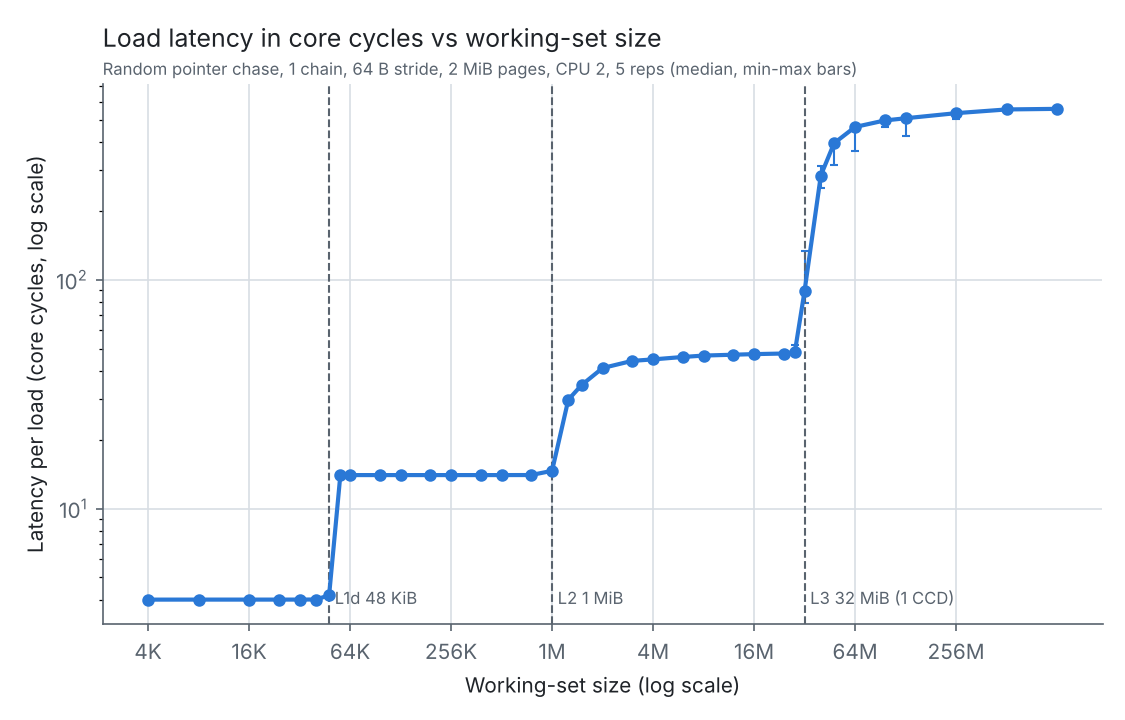
\includegraphics[width=\linewidth,height=0.42\textheight,keepaspectratio]{p2_report_figures/ws_cycles.png}
\caption{Figure 1. Load latency in core cycles vs
working-set size (log--log), with cache capacities marked.}
\end{figure}

\begin{longtable}[]{@{}
  >{\raggedright\arraybackslash}p{(\columnwidth - 6\tabcolsep) * \real{0.2500}}
  >{\raggedright\arraybackslash}p{(\columnwidth - 6\tabcolsep) * \real{0.2500}}
  >{\raggedright\arraybackslash}p{(\columnwidth - 6\tabcolsep) * \real{0.2500}}
  >{\raggedright\arraybackslash}p{(\columnwidth - 6\tabcolsep) * \real{0.2500}}@{}}
\toprule\noalign{}
\begin{minipage}[b]{\linewidth}\raggedright
Region
\end{minipage} & \begin{minipage}[b]{\linewidth}\raggedright
Sizes
\end{minipage} & \begin{minipage}[b]{\linewidth}\raggedright
Cycles
\end{minipage} & \begin{minipage}[b]{\linewidth}\raggedright
Interpretation
\end{minipage} \\
\midrule\noalign{}
\endhead
\bottomrule\noalign{}
\endlastfoot
L1 & 4--40 KiB & 4.0 & Fits in 48 KiB L1 \\
L1 edge & 48 KiB & 4.2 & At capacity; stack and other data
compete \\
L2 & 56--768 KiB & 14.0 & Flat \\
L2 $\rightarrow$ L3 & 1--3 MiB & 14.6 $\rightarrow$ 44 & Gradual \\
L3 & 4--28 MiB & 45--48.5 & Mostly L3 \\
L3 $\rightarrow$ DRAM & 32--64 MiB & 79 $\rightarrow$ 460 & Step just past 32 MiB \\
DRAM & 128 MiB--1 GiB & 507 $\rightarrow$ 558 & Approaches pure DRAM \\
\end{longtable}

\textbf{One CCD's L3, not 64 MiB.} The third step is at 32
MiB. The chip has 64 MiB of L3, but a thread on CCD 0 only
uses its own CCD's 32 MiB.

\textbf{AMAT and the gradual transitions.} Using AMAT =
\emph{h}$\cdot$\emph{t}\textsubscript{fast} + (1 $-$
\emph{h})$\cdot$\emph{t}\textsubscript{slow} with the plateau
values, I solved for the fraction \emph{h} of loads still
served by the faster level:

\begin{longtable}[]{@{}
  >{\raggedright\arraybackslash}p{(\columnwidth - 6\tabcolsep) * \real{0.2500}}
  >{\raggedright\arraybackslash}p{(\columnwidth - 6\tabcolsep) * \real{0.2500}}
  >{\raggedright\arraybackslash}p{(\columnwidth - 6\tabcolsep) * \real{0.2500}}
  >{\raggedright\arraybackslash}p{(\columnwidth - 6\tabcolsep) * \real{0.2500}}@{}}
\toprule\noalign{}
\begin{minipage}[b]{\linewidth}\raggedright
Size
\end{minipage} & \begin{minipage}[b]{\linewidth}\raggedright
Measured
\end{minipage} & \begin{minipage}[b]{\linewidth}\raggedright
Inferred hit fraction \emph{h}
\end{minipage} & \begin{minipage}[b]{\linewidth}\raggedright
Capacity ratio
\end{minipage} \\
\midrule\noalign{}
\endhead
\bottomrule\noalign{}
\endlastfoot
1.25 MiB & 30.2 cycles & 0.51 in L2 & 0.80 \\
1.5 MiB & 34.6 & 0.38 & 0.67 \\
2 MiB & 41.1 & 0.19 & 0.50 \\
40 MiB & 284 & 0.54 in L3 & 0.80 \\
64 MiB & 460 & 0.19 & 0.50 \\
256 MiB & 533 & 0.05 & 0.13 \\
\end{longtable}

A cyclic chain larger than the cache would get \emph{h} = 0
under pure LRU replacement and \emph{h} = capacity ratio
under ideal replacement. The measured values lie in between,
at 0.37--0.67 of the capacity ratio, which is consistent
with an adaptive or partly random replacement policy (an
inference, not a measurement).

\textbf{Order check.} In cycles, the three sessions differ
by a median of \textbf{0.09\%} per size. The largest
difference, 14\%, is at 32 MiB, exactly at the L3 edge,
where small changes in what else occupies L3 matter most.
dTLB misses were 0.000 at every size because the runs used 2
MiB pages (even 1 GiB is only 512 pages).

\hypertarget{pattern-and-granularity-sweep}{%
\subsection{6. Pattern and granularity
sweep}\label{pattern-and-granularity-sweep}}

1 GiB working set (DRAM), CPU 2, 5 repetitions. Latency from
\texttt{pchase}, bandwidth from \texttt{bwbench} (1 thread,
reads).

\begin{longtable}[]{@{}
  >{\raggedright\arraybackslash}p{(\columnwidth - 10\tabcolsep) * \real{0.1667}}
  >{\raggedright\arraybackslash}p{(\columnwidth - 10\tabcolsep) * \real{0.1667}}
  >{\raggedright\arraybackslash}p{(\columnwidth - 10\tabcolsep) * \real{0.1667}}
  >{\raggedright\arraybackslash}p{(\columnwidth - 10\tabcolsep) * \real{0.1667}}
  >{\raggedright\arraybackslash}p{(\columnwidth - 10\tabcolsep) * \real{0.1667}}
  >{\raggedright\arraybackslash}p{(\columnwidth - 10\tabcolsep) * \real{0.1667}}@{}}
\toprule\noalign{}
\begin{minipage}[b]{\linewidth}\raggedright
Stride
\end{minipage} & \begin{minipage}[b]{\linewidth}\raggedright
Seq latency
\end{minipage} & \begin{minipage}[b]{\linewidth}\raggedright
Random latency
\end{minipage} & \begin{minipage}[b]{\linewidth}\raggedright
Seq advantage
\end{minipage} & \begin{minipage}[b]{\linewidth}\raggedright
Seq bandwidth
\end{minipage} & \begin{minipage}[b]{\linewidth}\raggedright
Random bandwidth
\end{minipage} \\
\midrule\noalign{}
\endhead
\bottomrule\noalign{}
\endlastfoot
64 B & 1.22 ns (5.3 cyc) & 97.8 ns & 80$\times$ & \textbf{54.0
GB/s} & 4.29 GB/s \\
256 B & 2.96 ns (12.9 cyc) & 100.2 ns & 34$\times$ & 14.8 GB/s &
4.31 GB/s \\
1024 B & 4.54 ns (19.8 cyc) & 98.8 ns & 22$\times$ & 14.1 GB/s &
4.26 GB/s \\
\end{longtable}

\begin{figure}
\centering
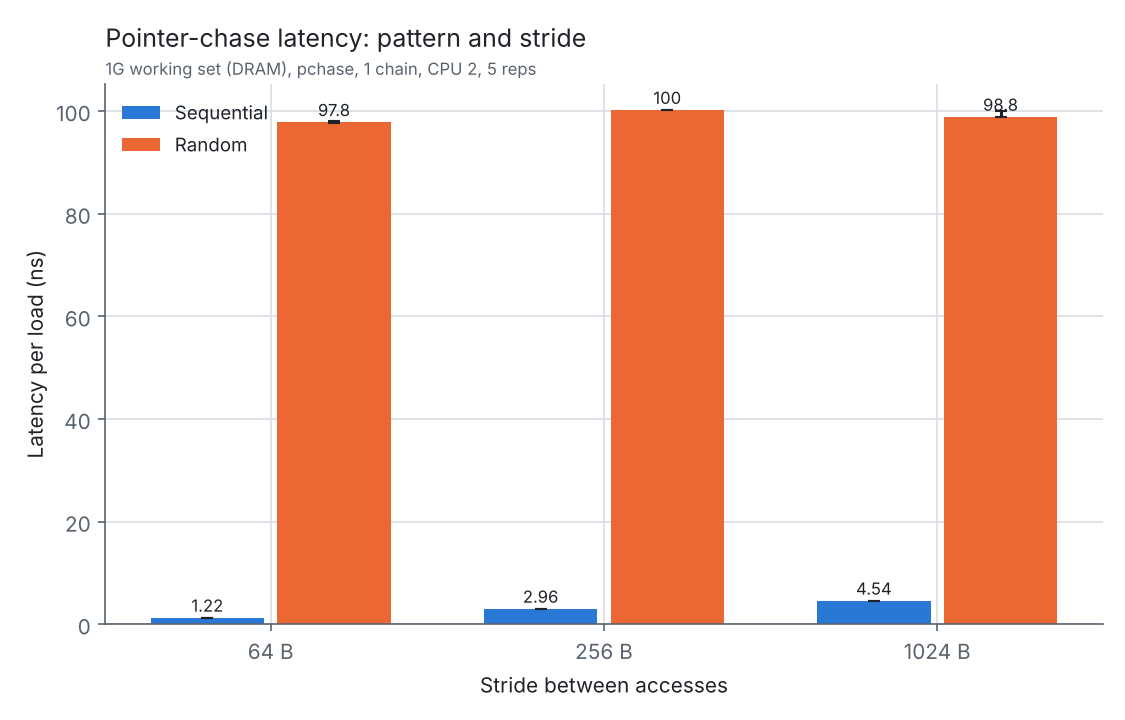
\includegraphics[width=\linewidth,height=0.42\textheight,keepaspectratio]{p2_report_figures/pattern_latency.png}
\caption{Figure 2. Pointer-chase latency by pattern and
stride (1 GiB).}
\end{figure}

\begin{figure}
\centering
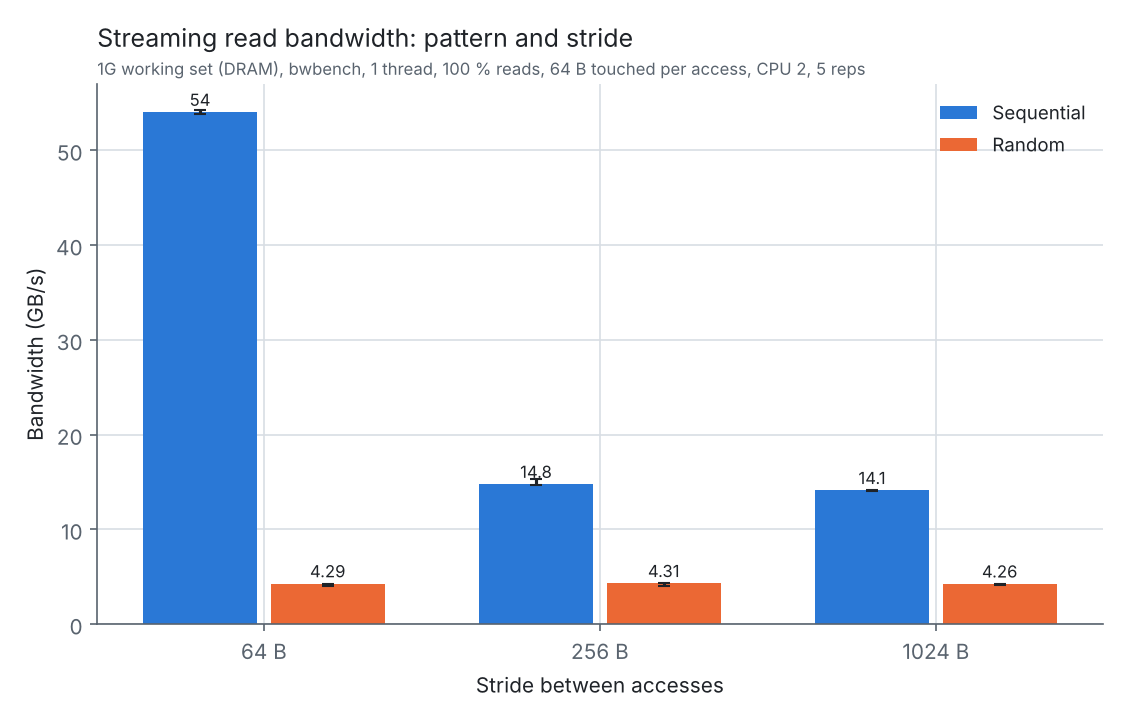
\includegraphics[width=\linewidth,height=0.42\textheight,keepaspectratio]{p2_report_figures/pattern_bw.png}
\caption{Figure 3. Single-thread read bandwidth by pattern
and stride (1 GiB).}
\end{figure}

\textbf{Random is $\sim$98 ns at every stride}:
each access is a DRAM miss, so only order matters.
\textbf{Sequential slows as the stride grows but stays far
below DRAM latency}: at 64 B prefetched lines are waiting in
L1 (5.3 cycles); at 256 B they arrive at about L2 latency
(12.9 vs 14 cycles); at 1024 B somewhere between L2 and L3.
The prefetchers detect even a 1 KiB stride but run less far
ahead.

\textbf{Little's Law on bandwidth.} Outstanding misses =
(bytes/s ÷ 64 B) $\times$ latency:

\begin{itemize}
\tightlist
\item
  Random: 4.29 GB/s ÷ 64 B = 67 M lines/s $\times$ 98 ns $\approx$
  \textbf{7 misses in flight}. Without prefetching, overlap
  comes only from the out-of-order window looking ahead in
  the loop; $\sim$7 is consistent with a few dozen
  instructions per chunk.
\item
  Sequential at 256--1024 B: $\sim$14.5 GB/s $\rightarrow$ 226
  M/s $\times$ 98 ns $\approx$ \textbf{22}, flat across strides, so stride
  is not the limit. This is how far the prefetcher runs
  ahead. (I first misread it as the core's limit; §8
  measured that directly as $\sim$48.)
\end{itemize}

\hypertarget{readwrite-mix-sweep}{%
\subsection{7. Read/write mix
sweep}\label{readwrite-mix-sweep}}

Sequential, 64 B stride, 1 GiB, 1 and 16 threads, 5
repetitions. \texttt{gb\_per\_s} counts each chunk once.

\begin{longtable}[]{@{}
  >{\raggedright\arraybackslash}p{(\columnwidth - 6\tabcolsep) * \real{0.2500}}
  >{\raggedright\arraybackslash}p{(\columnwidth - 6\tabcolsep) * \real{0.2500}}
  >{\raggedright\arraybackslash}p{(\columnwidth - 6\tabcolsep) * \real{0.2500}}
  >{\raggedright\arraybackslash}p{(\columnwidth - 6\tabcolsep) * \real{0.2500}}@{}}
\toprule\noalign{}
\begin{minipage}[b]{\linewidth}\raggedright
Mix
\end{minipage} & \begin{minipage}[b]{\linewidth}\raggedright
1 thread
\end{minipage} & \begin{minipage}[b]{\linewidth}\raggedright
16 threads
\end{minipage} & \begin{minipage}[b]{\linewidth}\raggedright
Estimated DRAM traffic (1 thread)
\end{minipage} \\
\midrule\noalign{}
\endhead
\bottomrule\noalign{}
\endlastfoot
100\% read & 54.1 GB/s & 48.3 GB/s & 54.1 \\
70/30 & 35.2 & 33.9 & 0.7$\cdot$35.2 + 0.3$\cdot$35.2$\cdot$\textbf{2} =
45.8 \\
50/50 & 28.8 & 29.0 & 14.4 + 28.8 = 43.2 \\
100\% write & 22.4 & 22.7 & 22.4$\cdot$\textbf{2} = 44.8 \\
\end{longtable}

\begin{figure}
\centering
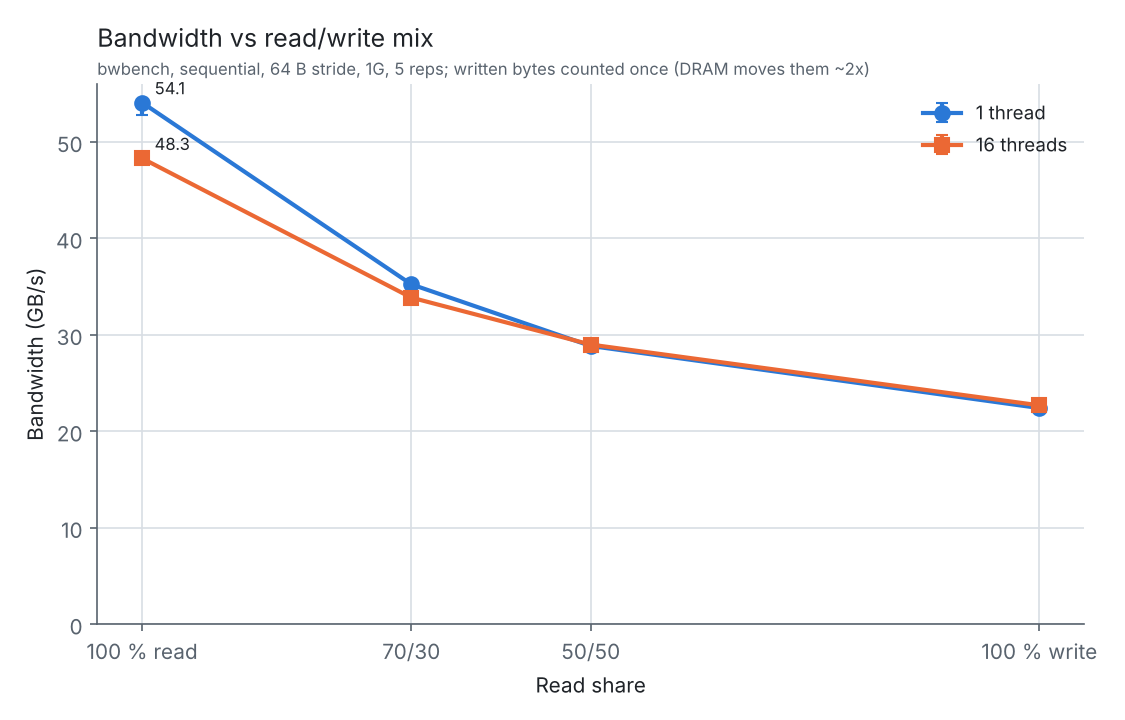
\includegraphics[width=\linewidth,height=0.42\textheight,keepaspectratio]{p2_report_figures/rw_bw.png}
\caption{Figure 4. Bandwidth vs read share for 1 and 16
threads.}
\end{figure}

Bandwidth falls as the write share rises. A normal store
first reads the line into the cache (read-for-ownership) and
later writes the whole line back, so each written byte
crosses the memory bus twice. Counting that, \textbf{DRAM
traffic stays at 43--54 GB/s for every mix}: memory moves
about the same number of bytes per second, but writes need
twice as many per useful byte. Mixed traffic is slightly
below pure reads, consistent with the cost of turning the
bus around between reads and writes. One thread already
saturates memory; 16 threads are no faster, and slightly
slower for pure reads (48.3 vs 54.1 GB/s), consistent with
many interleaved streams breaking up DRAM row locality.
Latency under each mix was not measured (§13).

\hypertarget{intensity-sweep-the-knee-and-littles-law}{%
\subsection{8. Intensity sweep: the knee and Little's
Law}\label{intensity-sweep-the-knee-and-littles-law}}

\hypertarget{memory-level-parallelism-on-one-core}{%
\subsubsection{8.1 Memory-level parallelism on one
core}\label{memory-level-parallelism-on-one-core}}

One thread on CPU 2, \emph{k} independent random chains over
1 GiB. Per-chain latency = ns per load $\times$ \emph{k}; bandwidth
= 64 B ÷ ns.

\begin{longtable}[]{@{}
  >{\raggedright\arraybackslash}p{(\columnwidth - 6\tabcolsep) * \real{0.2500}}
  >{\raggedright\arraybackslash}p{(\columnwidth - 6\tabcolsep) * \real{0.2500}}
  >{\raggedright\arraybackslash}p{(\columnwidth - 6\tabcolsep) * \real{0.2500}}
  >{\raggedright\arraybackslash}p{(\columnwidth - 6\tabcolsep) * \real{0.2500}}@{}}
\toprule\noalign{}
\begin{minipage}[b]{\linewidth}\raggedright
\emph{k}
\end{minipage} & \begin{minipage}[b]{\linewidth}\raggedright
Latency per load
\end{minipage} & \begin{minipage}[b]{\linewidth}\raggedright
Bandwidth
\end{minipage} & \begin{minipage}[b]{\linewidth}\raggedright
Gain vs previous point
\end{minipage} \\
\midrule\noalign{}
\endhead
\bottomrule\noalign{}
\endlastfoot
1 & 99.2 ns & 0.65 GB/s & \\
8 & 104.7 & 4.89 & \\
16 & 110.3 & 9.29 & \\
32 & 122.4 & 16.7 & \\
40 & 128.1 & 20.0 & +19\% for +25\% chains \\
48 & 134.7 & 22.8 & +14\% for +20\% chains \\
\textbf{64} & \textbf{158.6} & \textbf{25.8} & \textbf{+13\%
for +33\% chains} \\
\end{longtable}

\begin{figure}
\centering
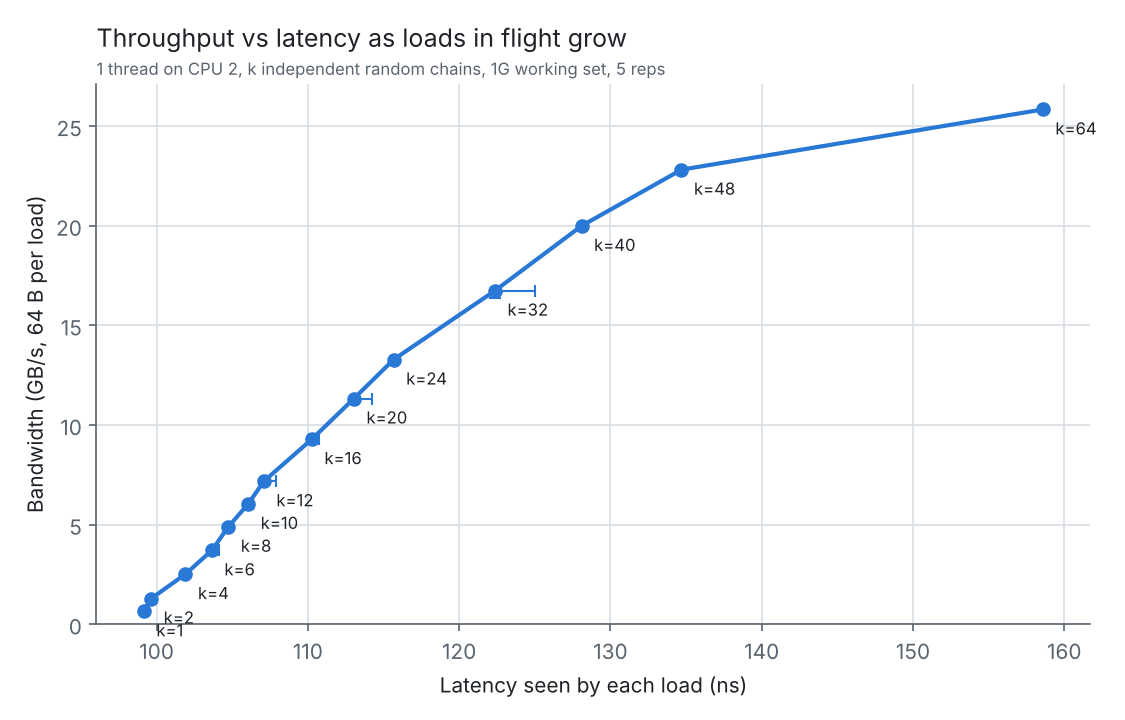
\includegraphics[width=\linewidth,height=0.42\textheight,keepaspectratio]{p2_report_figures/mlp_tradeoff.png}
\caption{Figure 5. Bandwidth vs per-load latency as
independent chains grow (the knee).}
\end{figure}

\textbf{The knee is between 48 and 64 chains.} Up to 32
chains, doubling the chains nearly doubles bandwidth while
latency rises only 23\%. From 48 to 64, a third more chains
buys 13\% more bandwidth while latency jumps by 24 ns, more
than over the whole range 1--32: extra requests now mostly
wait in line. One core reaches about \textbf{26 GB/s with
random accesses}, half of its 54 GB/s sequential rate,
because prefetchers issue requests from L2 without being
limited by what the core can track.

\textbf{Little's Law.} Throughput = outstanding requests ÷
latency. Here the number of outstanding misses is set
directly (\emph{k}), so the law describes the curve: while
latency stays near 99 ns, bandwidth grows in proportion to
\emph{k}; once queueing raises the latency, the same added
requests buy proportionally less (at \emph{k} = 64: 64 $\times$ 64
B ÷ 158.6 ns = 25.8 GB/s, instead of 41 GB/s at idle
latency). In this benchmark the law cannot be \emph{tested},
because latency and bandwidth are both derived from the same
time per load. Independent checks come from the other
benchmarks: \texttt{bwbench} random order ($\approx$7 in flight, §6)
and random SAXPY ($\approx$34 in flight at 1 GiB, matching the
32-chain point, §9). The \emph{k} = 1--32 points repeat the
first session within 1.4\%. Above $\sim$14 chains
some chain pointers spill to the stack, and at 64 the loop
is $\sim$200 instructions, so the knee may be
partly set by the instruction window rather than only the
miss buffers.

\hypertarget{loaded-latency}{%
\subsubsection{8.2 Loaded latency}\label{loaded-latency}}

A single-chain probe on CPU 15 (CCD 1) measured latency
while \texttt{bwbench} streamed reads on CPUs 0 \ldots{}
N$-$1.

\begin{longtable}[]{@{}lll@{}}
\toprule\noalign{}
Background cores & Background bandwidth & Probe latency \\
\midrule\noalign{}
\endhead
\bottomrule\noalign{}
\endlastfoot
0 & --- & 101 ns \\
1 & 55.0 GB/s & \textbf{423 ns} \\
2 & 51.6 & 271 \\
4 / 6 / 8 & 48.1 / 48.0 / 47.9 & 148 / 148 / 147 \\
10 / 12 / 14 & 47.6 / 47.6 / 47.6 & 176 / 203 / 233 \\
\end{longtable}

\begin{figure}
\centering
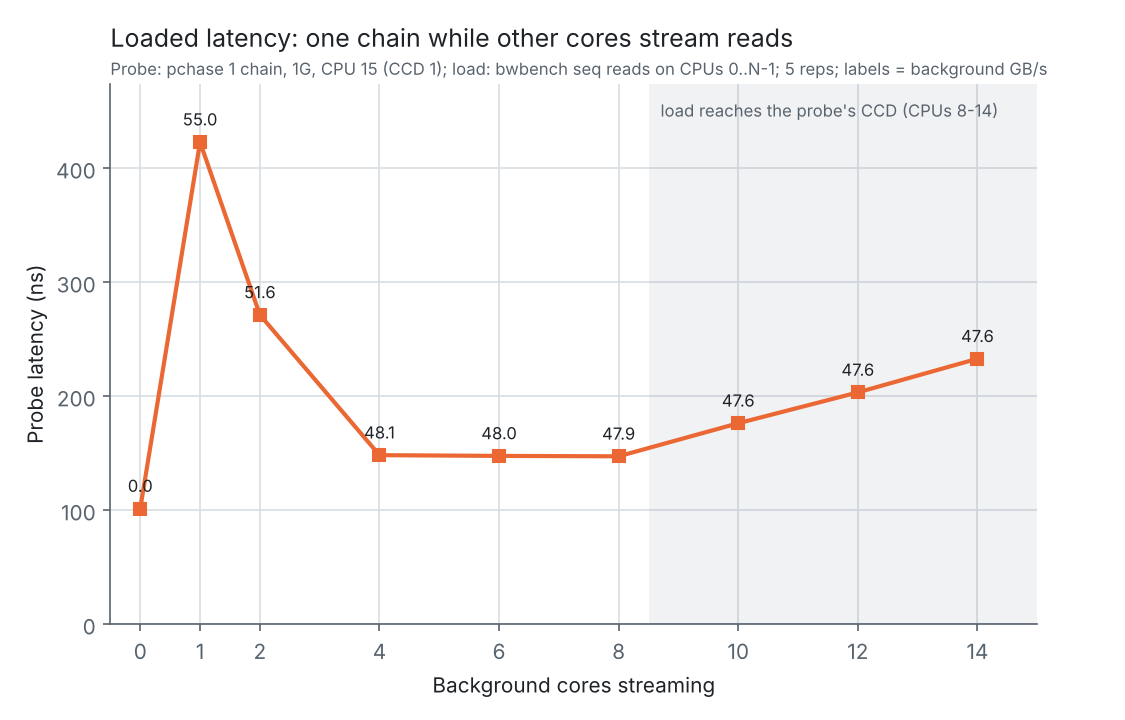
\includegraphics[width=\linewidth,height=0.42\textheight,keepaspectratio]{p2_report_figures/loaded_latency.png}
\caption{Figure 6. Probe latency vs number of background
cores; labels give background bandwidth.}
\end{figure}

\textbf{Latency follows how hard memory is driven, not how
many cores are busy.} One streaming core pulled the most
bandwidth (55 GB/s), and the probe waited longest. With 4--8
cores the total settled at $\sim$48 GB/s and
latency fell to 148 ns. Near saturation, a 15\% rise in
bandwidth nearly tripled latency: the queueing knee.
\textbf{From 10 cores on}, bandwidth is flat but latency
rises again. That is exactly where background threads move
onto CPUs 8--14, the probe's own CCD, and share its link to
memory, which is a second place where requests queue. Both
explanations fit the data but were not isolated separately
(§16.3).

\hypertarget{cache-miss-impact-saxpy}{%
\subsection{9. Cache-miss impact
(SAXPY)}\label{cache-miss-impact-saxpy}}

\texttt{y\ =\ a$\cdot$x\ +\ y}, footprint (x + y) 16 KiB--1 GiB,
CPU 2, 2 MiB pages, 5 repetitions. ``L2 miss'' is perf's
generic \texttt{cache-misses} event, which Linux maps to L2
misses on AMD Zen (§12).

\begin{longtable}[]{@{}
  >{\raggedright\arraybackslash}p{(\columnwidth - 12\tabcolsep) * \real{0.1429}}
  >{\raggedright\arraybackslash}p{(\columnwidth - 12\tabcolsep) * \real{0.1429}}
  >{\raggedright\arraybackslash}p{(\columnwidth - 12\tabcolsep) * \real{0.1429}}
  >{\raggedright\arraybackslash}p{(\columnwidth - 12\tabcolsep) * \real{0.1429}}
  >{\raggedright\arraybackslash}p{(\columnwidth - 12\tabcolsep) * \real{0.1429}}
  >{\raggedright\arraybackslash}p{(\columnwidth - 12\tabcolsep) * \real{0.1429}}
  >{\raggedright\arraybackslash}p{(\columnwidth - 12\tabcolsep) * \real{0.1429}}@{}}
\toprule\noalign{}
\begin{minipage}[b]{\linewidth}\raggedright
Order
\end{minipage} & \begin{minipage}[b]{\linewidth}\raggedright
Footprint
\end{minipage} & \begin{minipage}[b]{\linewidth}\raggedright
ns/elem
\end{minipage} & \begin{minipage}[b]{\linewidth}\raggedright
IPC
\end{minipage} & \begin{minipage}[b]{\linewidth}\raggedright
L1D miss/elem
\end{minipage} & \begin{minipage}[b]{\linewidth}\raggedright
L2 miss/elem
\end{minipage} & \begin{minipage}[b]{\linewidth}\raggedright
GB/s (12 B/elem)
\end{minipage} \\
\midrule\noalign{}
\endhead
\bottomrule\noalign{}
\endlastfoot
seq & 16 KiB & 0.023 & 3.77 & 0.001 & 0.000 & 516 \\
seq & 512 KiB & 0.030 & 2.87 & 0.125 & 0.000 & 400 \\
seq & 16 MiB & 0.069 & 1.25 & 0.126 & 0.016 & 175 \\
seq & 1 GiB & 0.269 & 0.32 & 0.127 & 0.002 &
\textbf{44.7} \\
rand & 16 KiB & 0.352 & 4.55 & 0.000 & 0.000 & 34.0 \\
rand & 512 KiB & 0.482 & 3.32 & 1.90 & 0.000 & 24.9 \\
rand & 16 MiB & 0.974 & 1.65 & 2.06 & 1.94 & 12.3 \\
rand & 48 MiB & 3.84 & 0.42 & 2.07 & 2.00 & 3.1 \\
rand & 1 GiB & \textbf{6.01} & 0.20 & 2.09 & 2.06 & 2.0 \\
\end{longtable}

\emph{Selected rows; the full table is
\texttt{results/processed/saxpy.md}.}

\begin{figure}
\centering
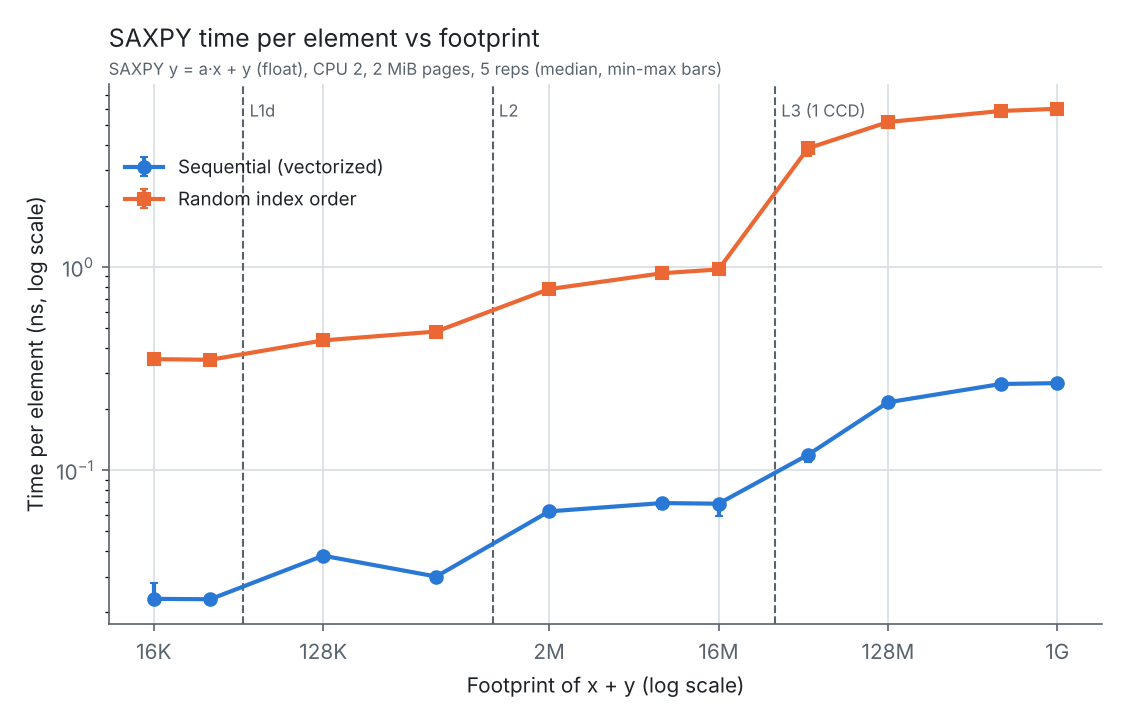
\includegraphics[width=\linewidth,height=0.42\textheight,keepaspectratio]{p2_report_figures/saxpy_runtime.png}
\caption{Figure 7. SAXPY time per element vs footprint,
sequential vs random order.}
\end{figure}

\begin{figure}
\centering
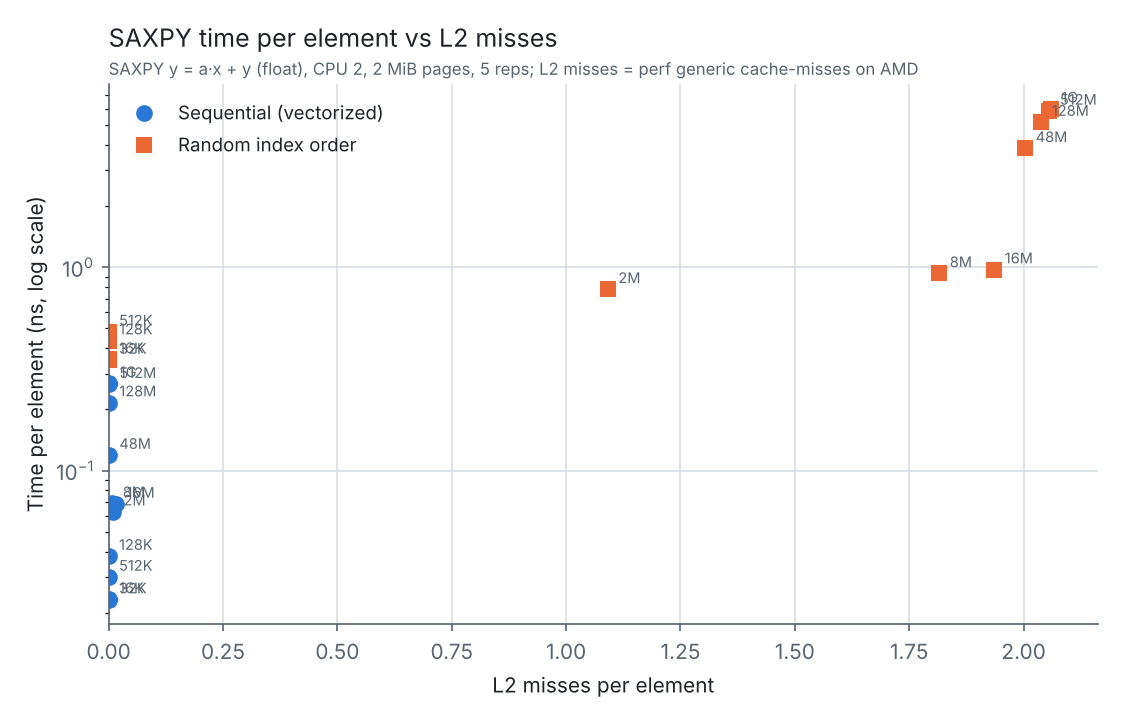
\includegraphics[width=\linewidth,height=0.42\textheight,keepaspectratio]{p2_report_figures/saxpy_misses.png}
\caption{Figure 8. Time per element vs L2 misses per
element.}
\end{figure}

\textbf{Sequential is bandwidth-bound at every level.} Time
per element steps from 0.023 ns (L1, $\sim$10
elements per cycle) to 0.27 ns in DRAM, where it moves 44.7
GB/s, the same ceiling as the read/write mixes in §7. L1D
misses are exactly 0.125 per element above L1 (2 lines per
16 elements), but \textbf{L2 misses stay near zero even at 1
GiB} while time grows 12$\times$: the prefetchers fetch the data
before the loop asks for it, so demand-miss counters see
hits. The correlation of time with L2 misses is therefore
\textbf{r = $-$0.17}.

\textbf{Random order is miss-bound.} Every element costs two
line misses (x{[}j{]} and y{[}j{]}). L2 misses rise from 0
to 2 per element as the footprint passes 1 MiB and explain
the climb up to 16 MiB (\textbf{r = 0.74}). The large jump
at 48 MiB happens with almost no change in L2 misses: the
misses are the same, but now DRAM serves them instead of L3,
which one counter cannot distinguish. At 1 GiB, 2.06 misses
per 6.01 ns at $\sim$98 ns each gives about
\textbf{34 misses in flight}, agreeing with §8.1 (32 chains:
3.82 ns per load). Random order moves two 64 B lines plus a
write-back for 12 useful bytes, so useful throughput is 22$\times$
lower than sequential.

\hypertarget{tlb-miss-impact}{%
\subsection{10. TLB-miss impact}\label{tlb-miss-impact}}

Random chase with a 4096 B stride (every access a new 4 KiB
page), 4 KiB vs 2 MiB pages, CPU 2, 5 repetitions.

\begin{longtable}[]{@{}
  >{\raggedright\arraybackslash}p{(\columnwidth - 12\tabcolsep) * \real{0.1429}}
  >{\raggedright\arraybackslash}p{(\columnwidth - 12\tabcolsep) * \real{0.1429}}
  >{\raggedright\arraybackslash}p{(\columnwidth - 12\tabcolsep) * \real{0.1429}}
  >{\raggedright\arraybackslash}p{(\columnwidth - 12\tabcolsep) * \real{0.1429}}
  >{\raggedright\arraybackslash}p{(\columnwidth - 12\tabcolsep) * \real{0.1429}}
  >{\raggedright\arraybackslash}p{(\columnwidth - 12\tabcolsep) * \real{0.1429}}
  >{\raggedright\arraybackslash}p{(\columnwidth - 12\tabcolsep) * \real{0.1429}}@{}}
\toprule\noalign{}
\begin{minipage}[b]{\linewidth}\raggedright
Region
\end{minipage} & \begin{minipage}[b]{\linewidth}\raggedright
Pages
\end{minipage} & \begin{minipage}[b]{\linewidth}\raggedright
Data footprint
\end{minipage} & \begin{minipage}[b]{\linewidth}\raggedright
2 MiB pages
\end{minipage} & \begin{minipage}[b]{\linewidth}\raggedright
4 KiB pages
\end{minipage} & \begin{minipage}[b]{\linewidth}\raggedright
dTLB miss/access (4 KiB)
\end{minipage} & \begin{minipage}[b]{\linewidth}\raggedright
Extra cycles per miss
\end{minipage} \\
\midrule\noalign{}
\endhead
\bottomrule\noalign{}
\endlastfoot
4 MiB & 1,024 & 64 KiB & 45.3 cyc & 31.6 cyc & 0.000 &
--- \\
16 MiB & 4,096 & 256 KiB & 45.4 & 55.8 & 0.128 &
$\sim$80 (few misses) \\
64 MiB & 16,384 & 1 MiB & 45.3 & 84.9 & 0.934 &
\textbf{42} \\
256 MiB & 65,536 & 4 MiB & 521.7 & 569.9 & 0.903 &
\textbf{53} \\
1 GiB & 262,144 & 16 MiB & 564.4 & 628.5 & 1.001 &
\textbf{64} \\
\end{longtable}

2 MiB pages had 0.000 dTLB misses at every size. L1D misses
were 1.000 per access for both page sizes.

\begin{figure}
\centering
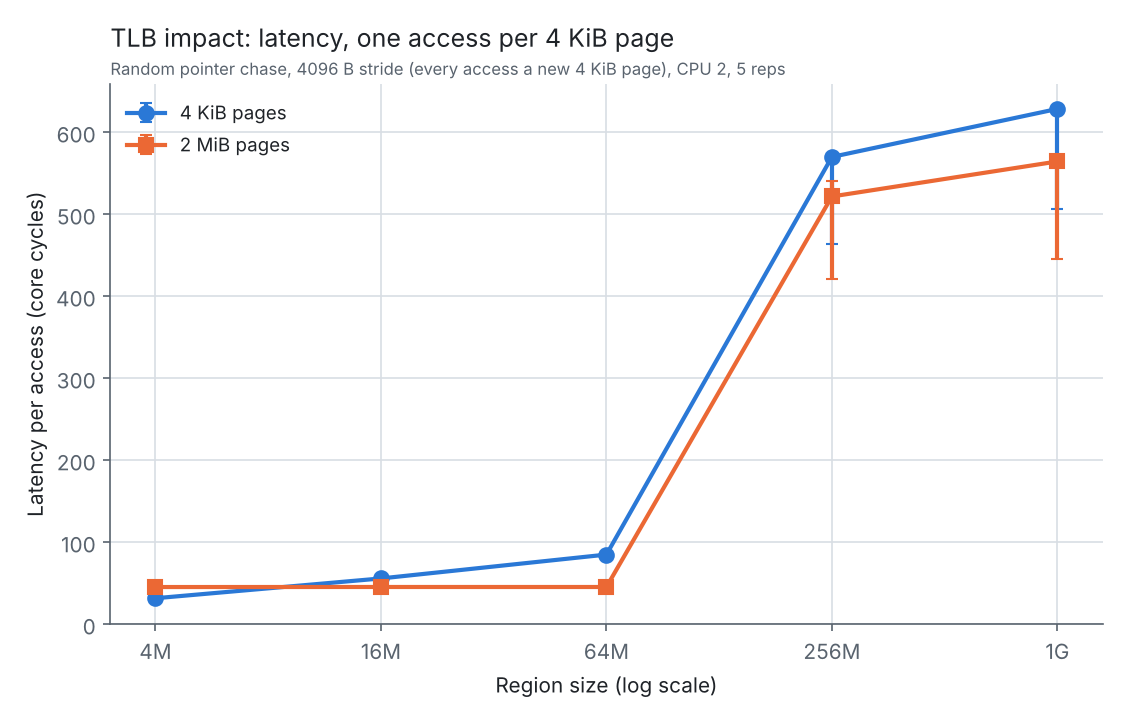
\includegraphics[width=\linewidth,height=0.42\textheight,keepaspectratio]{p2_report_figures/tlb_latency.png}
\caption{Figure 9. Latency per access (cycles), 4 KiB vs 2
MiB pages.}
\end{figure}

\begin{figure}
\centering
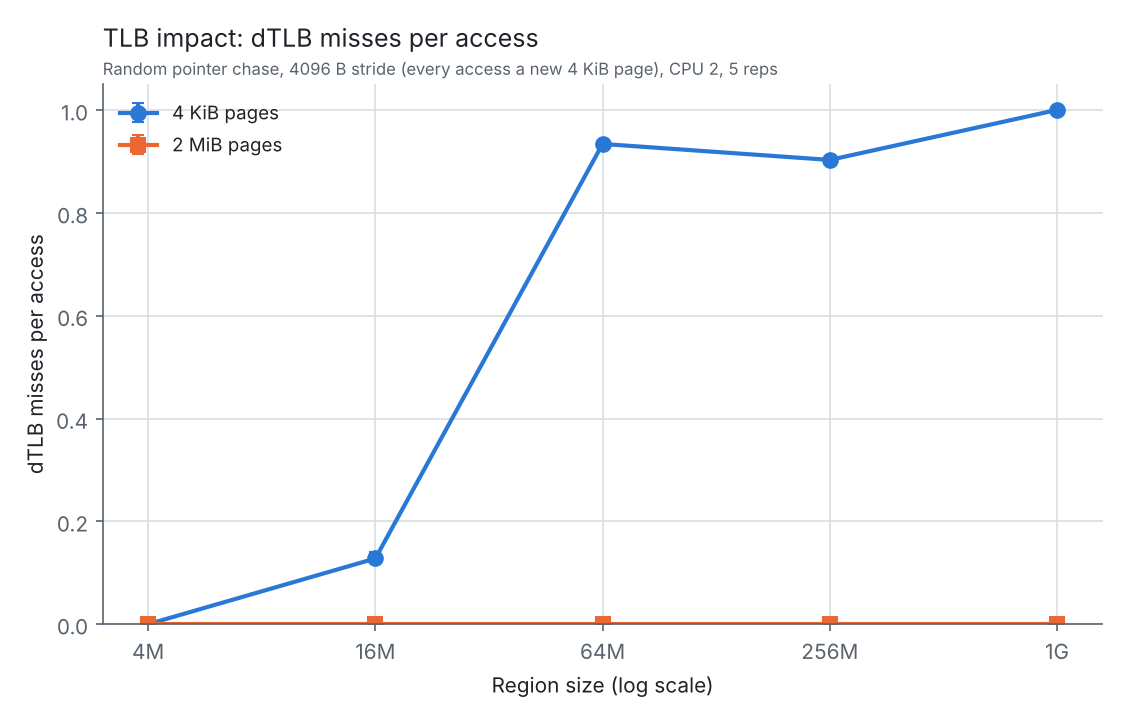
\includegraphics[width=\linewidth,height=0.42\textheight,keepaspectratio]{p2_report_figures/tlb_misses.png}
\caption{Figure 10. dTLB misses per access.}
\end{figure}

\textbf{TLB reach.} At 16 MiB, 87\% of 4,096 translations
still hit, so the TLB holds a few thousand 4 KiB entries
(about 3,500 if replacement were random), a reach of roughly
14 MiB. Beyond that, nearly every access walks the page
table.

\textbf{Cost of a miss.} Dividing the extra cycles by the
misses gives 42--64 cycles per miss, close to the 47-cycle
L3 latency: page-table entries are served from cache, not
DRAM. The cost grows with region size because the last-level
page table grows from 128 KiB (64 MiB region) to 2 MiB (1
GiB) and is pushed further out of cache. At 512 MiB (§11.2),
the same calculation gave 52 cycles per miss.

\textbf{Cache effects inside this test.} Because every line
sits at offset 0 of a page, all lines share the same low
address bits and crowd into a small fraction of the cache
sets: L1D misses are 1.000 per access even at 4 MiB (64 KiB
of data), and with 2 MiB pages nothing is served from L2 (45
cycles = L3) until 256 MiB, where accesses go to DRAM. This
is the same problem as walking down a column of a matrix
whose rows are 4 KiB long. The 4 MiB anomaly, where 4 KiB
pages are faster, is explained in §12.

\hypertarget{benchmark-pitfalls-and-misleading-setups}{%
\subsection{11. Benchmark pitfalls and misleading
setups}\label{benchmark-pitfalls-and-misleading-setups}}

\hypertarget{sequential-pointer-chase-measures-the-prefetcher-not-dram}{%
\subsubsection{11.1 Sequential pointer chase measures the
prefetcher, not
DRAM}\label{sequential-pointer-chase-measures-the-prefetcher-not-dram}}

At 1 GiB, a sequential chase took \textbf{1.22 ns} per load
and a random chase \textbf{99.05 ns}: 81$\times$ apart. A naive
latency test that walks memory in order would report ``DRAM
latency $\approx$ 1 ns''.

\hypertarget{transparent-huge-pages-hide-tlb-misses}{%
\subsubsection{11.2 Transparent huge pages hide TLB
misses}\label{transparent-huge-pages-hide-tlb-misses}}

With THP set to \texttt{always}, a one-access-per-page test
at 512 MiB that does not request 4 KiB pages silently got
huge pages for the entire buffer (\texttt{AnonHugePages} =
524,288 kB) and recorded \textbf{0.000} dTLB misses per
access. Forcing 4 KiB pages with \texttt{MADV\_NOHUGEPAGE}
gave \textbf{0.909} misses and 47 extra cycles per access
(607.6 vs 560.5). A TLB study written without this check
would conclude that TLB misses do not exist.

\hypertarget{page-aligned-strides-measure-cache-set-conflicts}{%
\subsubsection{11.3 Page-aligned strides measure cache-set
conflicts}\label{page-aligned-strides-measure-cache-set-conflicts}}

§10: with a 4096 B stride, a 64 KiB data set misses L1 on
every access, and up to 1 MiB of data never fits in L2.

\hypertarget{miss-counters-do-not-see-prefetched-traffic}{%
\subsubsection{11.4 Miss counters do not see prefetched
traffic}\label{miss-counters-do-not-see-prefetched-traffic}}

§9: sequential SAXPY slowed 12$\times$ from L1 to DRAM with almost
no L2 demand misses (r = $-$0.17). Low miss counts do not mean
low memory cost.

\hypertarget{ai-generated-benchmark-code-that-compiled-ran-and-measured-the-wrong-thing}{%
\subsubsection{11.5 AI-generated benchmark code that
compiled, ran and measured the wrong
thing}\label{ai-generated-benchmark-code-that-compiled-ran-and-measured-the-wrong-thing}}

The first \texttt{pchase} kept the \emph{k} chain pointers
in a small array. It compiled and gave plausible numbers,
but \texttt{objdump} showed that GCC kept the array on the
stack and even vectorized it, so each step went through
memory, adding store-to-load forwarding latency, which would
inflate L1 latency. The kernels are now generated with one
register variable per chain, and \texttt{make\ check-asm}
checks the loop.

\hypertarget{frequency-scaling-distorts-nanosecond-comparisons}{%
\subsubsection{11.6 Frequency scaling distorts nanosecond
comparisons}\label{frequency-scaling-distorts-nanosecond-comparisons}}

§4: L3 latency varied 31\% in ns across 10 runs while cycles
varied 0.5\%, and L2 ran at 4.37 GHz while L1 and DRAM ran
at 5.71 GHz in the same session. Comparing cache levels in
ns would mix clock speed into the result.

\hypertarget{anomalies}{%
\subsection{12. Anomalies}\label{anomalies}}

\begin{enumerate}
\def\labelenumi{\arabic{enumi}.}
\tightlist
\item
  \textbf{Clock state follows the working set.} In all three
  working-set sessions, including the two in shuffled order,
  sizes up to 32 MiB ran at 4.37 GHz and sizes from 40 MiB
  up at 5.71 GHz. Since shuffling did not change it, the
  clock depends on the workload, not on when the point ran.
  The governor's reasons are not visible without root.
  Cycle-based results are unaffected.
\item
  \textbf{4 KiB pages faster than 2 MiB pages at 4 MiB}
  (31.6 vs 45.3 cycles) with zero dTLB misses for both. A
  \texttt{perf\ stat} check of L2 requests (20 M loads per
  rep) showed \textbf{57.6\%} L2 hits with 4 KiB pages vs
  \textbf{0.14\%} with 2 MiB pages. With one contiguous 2
  MiB page, the 1,024 lines have perfectly regular physical
  addresses and collide in the same L2 sets; scattered 4 KiB
  frames spread them out. AMD does not publish the L2
  set-index function, so the mechanism is a plausible
  explanation of a measured effect.
\item
  \textbf{perf \texttt{cache-misses} counts L2 misses on
  AMD.} I first labelled it ``LLC misses''. At a 2 MiB
  footprint, which fits in L3, random SAXPY showed 1.09
  misses per element; the count rises past L2's 1 MiB, not
  L3's 32 MiB. Labels were corrected; the data were
  unchanged.
\item
  \textbf{Loaded latency peaked with one background core}
  instead of rising steadily (§8.2): one prefetch-heavy
  stream drove memory harder than several.
\item
  \textbf{SAXPY sequential: 128 KiB slower than 512 KiB}
  (0.038 vs 0.030 ns per element). Both arrays are 2
  MiB-aligned, so \texttt{x{[}i{]}} and \texttt{y{[}i{]}}
  always map to the same cache sets; this known aliasing
  pattern is a possible cause, not tested.
\item
  \textbf{16 threads slower than 1 thread for pure reads}
  (48.3 vs 54.1 GB/s), discussed in §7.
\end{enumerate}

\hypertarget{limitations}{%
\subsection{13. Limitations}\label{limitations}}

\begin{itemize}
\tightlist
\item
  \textbf{No root access.} The governor and boost could not
  be fixed (results given in cycles and with the measured
  clock); hardware prefetchers could not be disabled
  (randomized order used instead); only user-space counters
  were available.
\item
  \textbf{No L3 (uncore) counters}, so true L3 misses were
  not measured. perf's \texttt{cache-misses} counts L2
  misses on AMD.
\item
  \textbf{Memory speed unknown.} The DDR5 speed grade and
  channel count need root (\texttt{dmidecode}), so bandwidth
  cannot be expressed as a fraction of the theoretical peak.
\item
  \textbf{Read/write mixes: throughput only.} The handout
  asks for latency under each mix as well; that was not
  measured.
\item
  \textbf{Intel MLC not used}; all latency and bandwidth
  numbers come from the custom benchmarks.
\item
  \textbf{Shared lab machine.} Sessions started with load
  averages of 0.06--0.72 and no other user jobs observed,
  but background activity cannot be ruled out.
\item
  \textbf{Repetitions within one process.} Each point's
  repetitions ran back-to-back in one process; separate
  sessions (working set $\times$3, chains $\times$2) agreed within
  0.1--1.4\%.
\item
  \textbf{Knee may include an instruction-window effect}
  above $\sim$14 chains (§8.1).
\end{itemize}

\hypertarget{reproducibility}{%
\subsection{14. Reproducibility}\label{reproducibility}}

\begin{verbatim}
make && make check-asm
python3 scripts/membench.py env
python3 scripts/membench.py run sanity baseline
python3 scripts/membench.py run ws
python3 scripts/membench.py run ws --shuffle --tag shuffled
python3 scripts/membench.py run pattern rw --shuffle
python3 scripts/membench.py run mlp loaded
python3 scripts/membench.py run mlp --tag k64
python3 scripts/membench.py run tlb --shuffle
python3 scripts/membench.py run saxpy
python3 scripts/membench.py parse
cd analysis && python3 plot_ws.py && python3 plot_sweeps.py && python3 plot_intensity.py && python3 plot_saxpy.py
\end{verbatim}

Raw output for every point, the exact command, environment
snapshot and hypothesis are in
\texttt{results/raw/\textless{}experiment\textgreater{}/\textless{}session\textgreater{}/};
\texttt{results/processed/} holds the per-repetition and
aggregated summaries.

\hypertarget{conclusion}{%
\subsection{15. Conclusion}\label{conclusion}}

The hierarchy behaves as documented in its fixed costs: 4,
14 and 47 cycles for L1, L2 and L3, and about 98 ns for
DRAM, with each step at the documented capacity and only one
CCD's 32 MiB of L3 visible to a thread. How much of that
cost a program actually pays depends on concurrency and
predictability. Sequential access hides DRAM latency almost
entirely (80$\times$ faster than random), one core can overlap
about 48 misses before its latency rises steeply, and near
saturation a small increase in bandwidth multiplies
everyone's latency. The same arithmetic in SAXPY ran 22$\times$
slower in random order. Several measurements also showed how
easily a benchmark can mislead: sequential chases,
transparent huge pages, page-aligned strides, demand-miss
counters and nanosecond comparisons under a changing clock
each gave a wrong answer until checked against a second
measurement.

\hypertarget{ai-use-note}{%
\subsection{16. AI-use note}\label{ai-use-note}}

I used Claude, an AI assistant from Anthropic, throughout
this project. It wrote all of the code, explained each step,
analyzed the results with me, and drafted this report and
the README. I ran every experiment on the lab machine over
SSH, and every number in this report comes from the raw
output stored in the repository. The AI read the results
from my project folder through a linked-computer connection
and regenerated the figures from them.

\hypertarget{division-of-work}{%
\subsubsection{16.1 Division of
work}\label{division-of-work}}

\begin{longtable}[]{@{}
  >{\raggedright\arraybackslash}p{(\columnwidth - 4\tabcolsep) * \real{0.3333}}
  >{\raggedright\arraybackslash}p{(\columnwidth - 4\tabcolsep) * \real{0.3333}}
  >{\raggedright\arraybackslash}p{(\columnwidth - 4\tabcolsep) * \real{0.3333}}@{}}
\toprule\noalign{}
\begin{minipage}[b]{\linewidth}\raggedright
Stage
\end{minipage} & \begin{minipage}[b]{\linewidth}\raggedright
What the AI did
\end{minipage} & \begin{minipage}[b]{\linewidth}\raggedright
What I did
\end{minipage} \\
\midrule\noalign{}
\endhead
\bottomrule\noalign{}
\endlastfoot
Learning & Explained latency vs bandwidth, prefetching, MLP,
Little's Law, AMAT, TLB reach, page walks & Asked questions
and chose the order of steps \\
Setup & Diagnosed the lack of root; gave the no-root perf
install (unpacking Arch packages) & Ran every command on the
lab machine and reported errors \\
Code & Wrote \texttt{pchase.c}, \texttt{bwbench.c},
\texttt{saxpy.c}, \texttt{membench.py}, the parser and
plotting scripts; tested them in its own Linux environment
before I ran them & Built and ran them on the real
machine \\
Experiment design & Proposed the matrix, hypotheses and
follow-ups (64 chains, perf L2 check, shuffled reruns) & Ran
all experiments, including the extra shuffled working-set
sessions \\
Analysis & Computed tables, Little's Law and AMAT estimates;
proposed interpretations & Reviewed results as they came
in \\
Writing & Drafted this report and the README & Reviewed and
edited them \\
\end{longtable}

\hypertarget{ai-errors-found-during-the-project}{%
\subsubsection{16.2 AI errors found during the
project}\label{ai-errors-found-during-the-project}}

\begin{longtable}[]{@{}
  >{\raggedright\arraybackslash}p{(\columnwidth - 6\tabcolsep) * \real{0.2500}}
  >{\raggedright\arraybackslash}p{(\columnwidth - 6\tabcolsep) * \real{0.2500}}
  >{\raggedright\arraybackslash}p{(\columnwidth - 6\tabcolsep) * \real{0.2500}}
  >{\raggedright\arraybackslash}p{(\columnwidth - 6\tabcolsep) * \real{0.2500}}@{}}
\toprule\noalign{}
\begin{minipage}[b]{\linewidth}\raggedright
\#
\end{minipage} & \begin{minipage}[b]{\linewidth}\raggedright
What the AI got wrong
\end{minipage} & \begin{minipage}[b]{\linewidth}\raggedright
How it was caught
\end{minipage} & \begin{minipage}[b]{\linewidth}\raggedright
Outcome
\end{minipage} \\
\midrule\noalign{}
\endhead
\bottomrule\noalign{}
\endlastfoot
1 & First \texttt{pchase} kept chain pointers in a stack
array (inflated latency) & The AI's own \texttt{objdump}
check & Kernels regenerated with one register per chain;
\texttt{make\ check-asm} added \\
2 & Called $\sim$22 outstanding misses (from
\texttt{bwbench}) the core's limit & The \texttt{mlp} sweep
showed no knee at 32 & Sweep extended to 64; knee found at
48--64; §6 corrected \\
3 & Labelled perf \texttt{cache-misses} as last-level-cache
misses & 1.09 misses/element at a 2 MiB footprint &
Relabelled as L2 misses (§12) \\
4 & Expected a large TLB penalty and treated 4 KiB vs 2 MiB
as a pure TLB comparison & Small penalty; 4 KiB faster at 4
MiB & Explained with cache-hit page walks and a perf L2
check (§10, §12) \\
5 & Predicted loaded latency would rise steadily with load &
Peak at one background core & Explained with the
background-bandwidth data (§8.2) \\
6 & Gave commands that failed: \texttt{/c/} paths in WSL,
\texttt{pip\ -\/-user} on Arch, the \texttt{libpfm4} package
name, \texttt{scp} to the machine's internal hostname & The
commands errored & Corrected commands given \\
7 & Produced figures with overlapping labels, a confusing
point order (loaded latency) and an overflowing subtitle &
Its own review of the rendered figures & Fixed and
regenerated \\
8 & Presented a ``Little's Law check'' figure for the chain
sweep as confirmation, although bandwidth and latency there
come from the same measurement, so the law holds identically
& The AI's own check of the report's numbers & Figure
removed; independent cross-benchmark checks used instead
(§8.1) \\
\end{longtable}

\hypertarget{claims-that-rest-on-the-ais-judgement}{%
\subsubsection{16.3 Claims that rest on the AI's
judgement}\label{claims-that-rest-on-the-ais-judgement}}

\begin{itemize}
\tightlist
\item
  The replacement-policy interpretation of the gradual steps
  (§5), the L2 placement explanation (§12.2), the CCD-link
  contention explanation (§8.2) and the clock-state
  behaviour (§12.1) are interpretations of the data, not
  isolated tests.
\item
  ``Commonly reported Zen 5 latencies'' for L1 and L2 come
  from the AI's knowledge, not a cited AMD document.
\item
  The $\sim$2$\times$ DRAM traffic for writes (§7) is a
  model (read-for-ownership plus write-back); DRAM traffic
  was not counted directly.
\end{itemize}

\end{document}
